\documentclass[tikz,border=2pt]{standalone}
\usepackage{amsmath}
\usetikzlibrary{arrows.meta}
\begin{document}
% Entry game: Out (0,2); after In the incumbent chooses A (1,1) or F (-1,-1). In the subgame
% after In only A is optimal, so the threat F is not credible; the unique SPNE is (In, A).
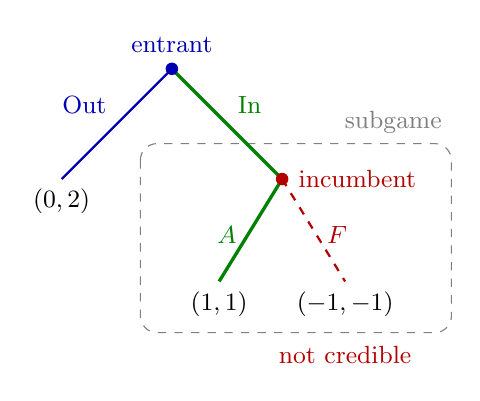
\begin{tikzpicture}[font=\small, >={Latex[length=2mm]},
    dec/.style={circle, fill, inner sep=1.6pt}]
  % subgame after In
  \draw[gray, dashed, rounded corners=6pt] (1.0,-0.95) rectangle (4.95,-3.35);
  \node[gray, anchor=south east] at (4.95,-0.95) {subgame};
  % edges (equilibrium path very thick green)
  \draw[thick, blue!70!black] (1.4,0) -- node[above left, pos=0.5] {Out} (0,-1.4);
  \draw[very thick, green!50!black] (1.4,0) -- node[above right, pos=0.5] {In} (2.8,-1.4);
  \draw[very thick, green!50!black] (2.8,-1.4) -- node[left, pos=0.55] {$A$} (2.0,-2.7);
  \draw[thick, red!70!black, dashed] (2.8,-1.4) -- node[right, pos=0.55] {$F$} (3.6,-2.7);
  % nodes
  \node[dec, blue!70!black, label={[blue!70!black]above:entrant}] at (1.4,0) {};
  \node[dec, red!70!black, label={[red!70!black]right:incumbent}] at (2.8,-1.4) {};
  % payoffs (entrant, incumbent)
  \node[anchor=north, inner sep=2pt] at (0,-1.45) {$(0,2)$};
  \node[anchor=north, inner sep=2pt] at (2.0,-2.75) {$(1,1)$};
  \node[anchor=north, inner sep=2pt] at (3.6,-2.75) {$(-1,-1)$};
  \node[red!70!black, anchor=north] at (3.6,-3.4) {not credible};
\end{tikzpicture}
\end{document}
